\chapter{Methodik}
\label{chap:methodik}

In diesem Kapitel wird der methodische Aufbau dieser Thesis beschrieben und begründet.
Die Arbeit ist als industrielle Fallstudie in Zusammenarbeit mit \emph{levigo solutions} konzipiert und dient der Evaluation des \gls{mmf} an einer bestehenden Microservices-Architektur.
Diese Fallstudie besteht aus zwei Hauptbestandteilen.
Im ersten Teil wird ein Refactoring des Produktes \emph{jadice flow} nach Anleitung des Frameworks durchgeführt.
Im zweiten Teil wird das Ergebnis dieses Refactorings verwendet, um eine Evaluation des Frameworks und Werkzeugs abzuschließen.

\section{Refactoring mit \gls{mmf}}

Die Vorgehensweise beim Refactoring ist durch das Framework sehr genau vorgegeben, daher wird das Refactoring in dieser Thesis in die gleichen drei Phasen unterteilt wie in \cref{sec:mmf} beschrieben.
In der ersten Phase wird ein Architekturreview nach \Citet{SVAHNBERG20071893} mit den Stakeholdern des Produkts durchgeführt.
Diese Methode wird in \cref{sec:methodik-architekturreview} näher beschrieben.
Das wesentliche Ergebnis dieses Reviews sind die gewünschten \glspl{qa} des Systems.
Diese Attribute sind die Basis für Phase 2 und 3 und werden in den \gls{arh} eingegeben.
Dieser führt Berechnungen mit den \glspl{qa} durch und kann so eine Liste von Refactoring-Methoden vorschlagen, die nach ihrer Eignung für die \glspl{qa} sortiert sind.
Als weitere Eingabe dafür dienen bestimmte Filter, die in \cref{sec:durchführung-phase2} näher erläutert werden.
Aus der resultierenden Liste von Migrationsmethoden werden die besten Vorschläge betrachtet und bewertet, bevor einer davon ausgewählt und in den folgenden Phasen verwendet wird.
Analog dazu wird in Phase 3a eine sortierte Liste von Patterns und Best Practices vorgeschlagen, ebenfalls durch Eingabe von \glspl{qa} und Filtern.
Das Vorgehen bei der Auswahl der Filter sowie die spätere Inspektion der Vorschläge des \gls{arh} werden in Form von strukturierten Feldnotizen protokolliert.
Deren genauere Funktion und Form dieser wird folgend in \cref{sec:structured-field-notes} erläutert.

\subsection{Architekturreview}
\label{sec:methodik-architekturreview}

Die Methodik eines Architekturreviews wird in dieser Thesis nach Vorschlag des \gls{mmf}/\gls{arh} dazu verwendet, Qualitätsanforderungen an das System, sogenannte \acrfullpl{qa}, zu sammeln.
Für Konformität mit dem Werkzeug \gls{arh}, das als Ergebnis des Architekturreviews Szenarien benötigt, die \acrfullpl{qa} beschreiben, beschränkt die Auswahl möglicher Verfahren für die erste Phase auf Szenarien-basierte Architekturreviews.
Das bedeutet, dass die gewünschten \glspl{qa} des Systems in Form von Szenarien erfasst und dokumentiert werden.
Dabei werden mit jedem Szenario zugehörige \glspl{qa} assoziiert, wodurch am Ende eine Abbildung aller \glspl{qa} auf ihre Priorität möglich ist.
Diese Abbildung ist das eigentliche Ergebnis, das der \gls{arh} als Eingabe für die weiteren Phasen benötigt.
Die Szenarien sind dabei lediglich ein Zwischenprodukt und sollen dabei helfen, eine genauere Vorstellung davon zu bekommen, welche spezifischen Situationen mit den \glspl{qa} verbunden sind.
Sie ermöglichen auch eine Bewertung der Wichtigkeit und technischen Schwierigkeit anhand konkreter Situationen, was bei abstrakten \glspl{qa} schwieriger wäre.

Geläufige Szenarien-basierte Verfahren sind die \gls{saam} nach \Citet{saam} und die \gls{atam} nach \Citet{kazman_2000}.
Da das Ausmaß dieser allerdings nicht angemessen für den Rahmen einer Thesis ist \cite{master-marvin-knodel}, würde für diese Arbeit höchstens eine stark abgewandelte Version dieser infrage kommen.
Stattdessen wurde sich in dieser Thesis für eine Modifikation des Architekturreviews nach \Citet{SVAHNBERG20071893} entschieden.
Dabei handelt es sich ebenfalls um eine Szenarien-basierte Methode, die auch auf \gls{saam} und \gls{atam} basiert, allerdings für kleinere Anwendungsfälle entworfen wurde.
Die Autoren beschreiben wie sie diese Methode zur Evaluation von Studentenprojekten verwenden, die ein reales Softwareentwicklungsprojekt mit Industriekunden nachahmen und einen Rahmen von 10-15 Teilnehmern und 20 Wochen Arbeitszeit haben.

Die vorgestellte Methodik für das Architekturreview nach  \Citet{SVAHNBERG20071893} besteht aus sechs Schritten (Übersicht in \cref{tab:svahnberg-plan}).
\begin{table}[!h]
  \centering
  \begin{tabular}{l l}
    \toprule
    \textbf{Aktivität} & \textbf{Zeit (in Minuten)} \\ \midrule
    1. Einleitung in das Projekt & 15 \\
    2. Identifikation von Qualitätsanforderungen & 20 \\
    3. Szenarienerhebung & 45 \\
    ~~~~Pause & 20 \\
    4. Architekturpräsentation & 20 \\
    5. Szenario- und Architekturanalyse & 90 \\
    6. Fazit & 15 \\
    \bottomrule
  \end{tabular}
  \caption[Zeitplan für ein Architekturreview nach \Citet{SVAHNBERG20071893}]{
    Zeitplan für ein Architekturreview nach \Citet{SVAHNBERG20071893}.
  }
  \label{tab:svahnberg-plan}
\end{table}

Diese sollen in einer etwa vierstündigen moderierten Gruppendiskussion mit den wichtigsten Stakeholdern des Produkts durchgeführt werden.
Im ersten Schritt gibt der \gls{po} eine Einführung in das Projekt, in der Ziele für das Produkt sowie die Organisation geschildert werden.
Danach beginnt im Schritt 2 die Identifikation der \glspl{qa} in einer Brainstorming-Runde mit Beteiligung von \gls{po}, End-Nutzer und Architekten.
Die Liste der Qualitätskriterien gemäß ISO 9126~\cite{ISO-9126} dient dabei als Vorlage für mögliche \glspl{qa}.
Im dritten Schritt ordnen \gls{po} und End-Nutzer die Liste der \glspl{qa} nach Wichtigkeit und fügen den drei wichtigsten jeweils zwei Szenarien hinzu.
Nach einer Pause präsentiert im vierten Schritt ein Softwarearchitekt die vorgeschlagene Architektur.
Anschließend werden im fünften Schritt die Szenarien nacheinander durchgegangen, analysiert und bewertet, inwiefern sie durch die Architektur erfüllt werden und wo etwaige Probleme bestehen.
Im sechsten Schritt werden alle festgestellten Probleme und Aspekte, die mehr Aufmerksamkeit benötigen, final diskutiert und der gesamte Prozess wird zusammengefasst.

Die vorgestellt Methodik wird in dieser Arbeit als Vorlage verwendet, muss nun allerdings noch auf den speziellen Anwendungsfall angepasst werden.
Während in \gls{saam}, \gls{atam} und dem Verfahren von \Citet{SVAHNBERG20071893} die Szenarien und \glspl{qa} lediglich ein Zwischenprodukt und Mittel zu Bewertung der Architektur des Systems sind, sind sie in dem Architekturreview, das im Rahmen dieser Thesis durchgeführt wird, das gewünschte Endprodukt.
Das bedeutet, dass die Schritte, die nach der Erhebung und Priorisierung der Szenarien erfolgen, also zur Evaluation des Systems, in diesem Fall nicht relevant sind und nicht durchgeführt werden.
Dabei handelt es sich um die Schritte 4,5 und 6, welche hauptsächlich der Bewertung des Systems unter den definierten \glspl{qa} dienen sollen.
Eine Ausnahme ist, dass \gls{mmf} und \gls{arh} einen Bewertungsschritt vorsehen, bei dem jedem Szenario zugeordnet wird, ob eine \gls{msa} für es profitabel ist.
Diese Bewertung könnte Schritt 5 zugeordnet werden.

Ein weiterer Unterschied zwischen diesem Anwendungsfall und dem von \Citet{SVAHNBERG20071893} beschriebenen erwarteten Anwendungsfällen ist, dass die Beschreibung des Projekts in Schritt 1 überflüssig ist.
Das liegt daran, dass die einzigen Stakeholder, die an dem Review teilnehmen der \acrfull{po} und vier Softwarearchitekten beziehungsweise -Entwickler sind, welche alle sehr gut mit dem Projekt vertraut sind und keine Einleitung benötigen.
Stattdessen wird in Schritt 1 eine Einleitung in die verwendete Methodik gegeben, da diese dem Team noch unbekannt war.

Somit bleiben im Wesentlichen neben dem veränderten Schritt 1 nur noch Schritt 2 und 3 für diesen Anwendungsfall übrig.
Diese wurden zusätzlich noch weiter auf die Verwendung mit dem \gls{arh} angepasst.
Im Schritt 2 werden als Basis-\glspl{qa} statt der ISO 9126~\cite{ISO-9126} die von \Citet{master-daniel-koch} speziell für Microservices-Architekturen identifizierten \glspl{qa} (siehe \cref{fig:qas}) verwendet.
\begin{figure}[!h]
	\centering
	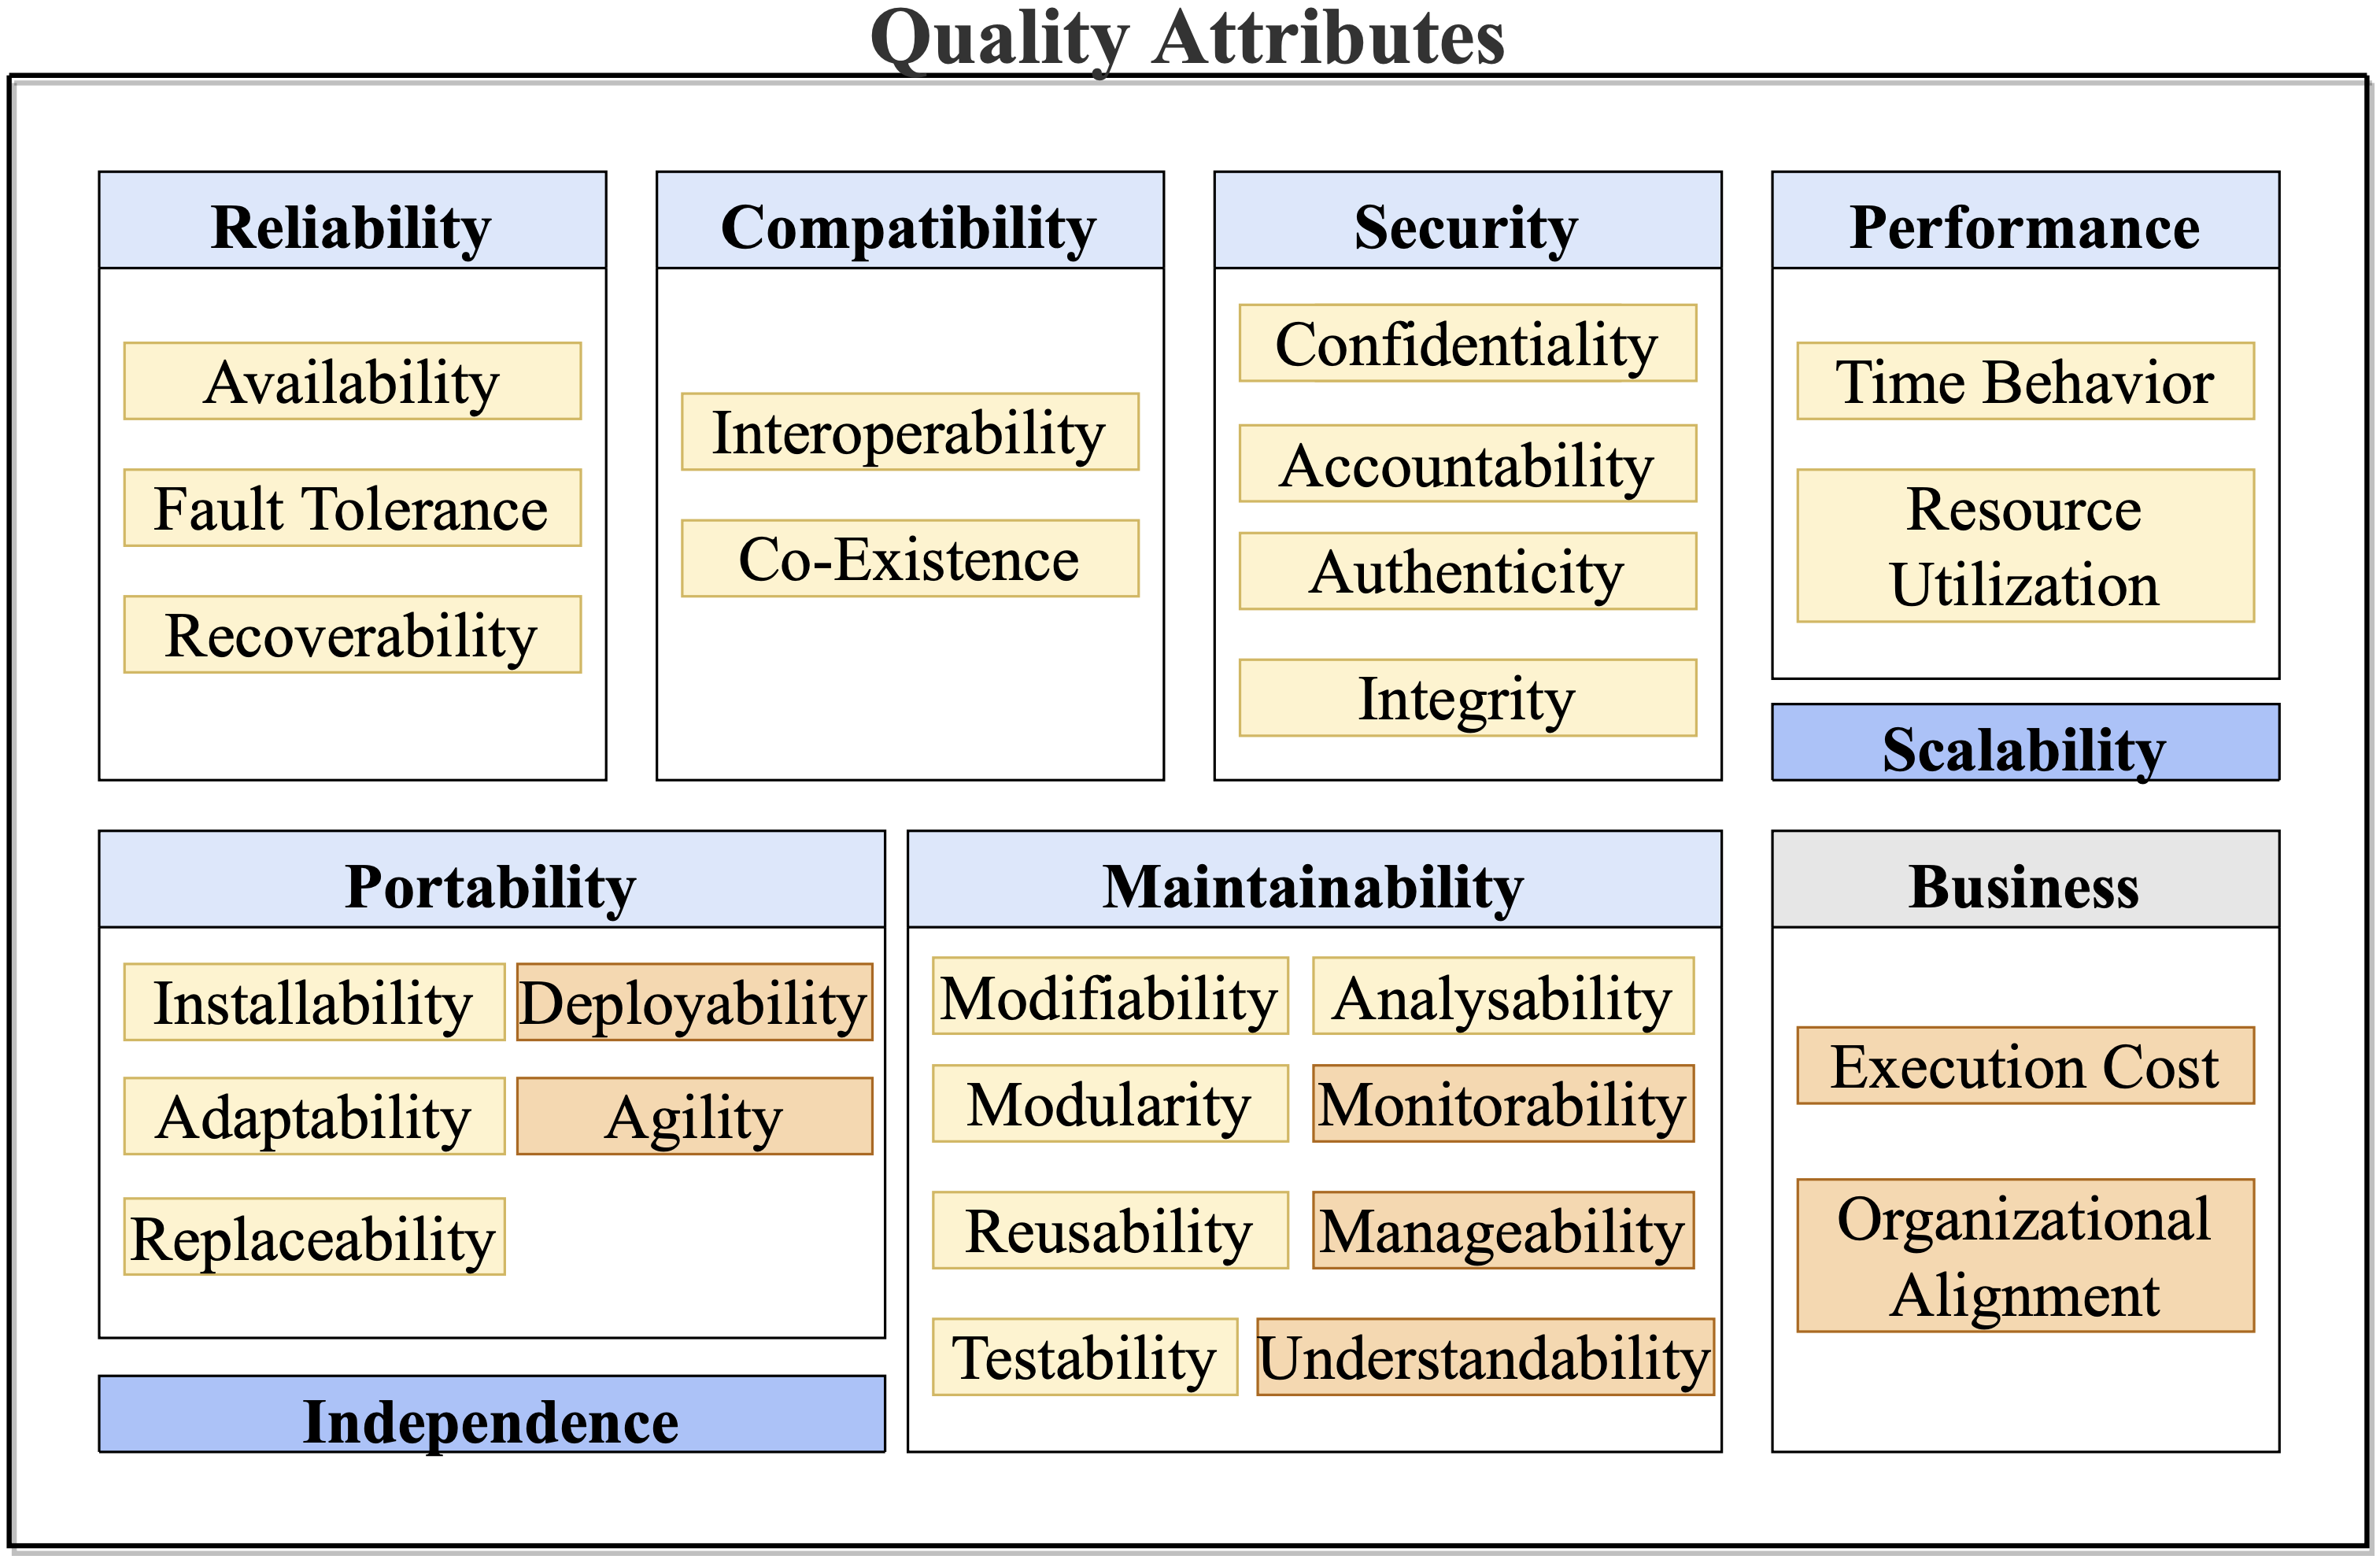
\includegraphics[width=\textwidth]{qas}
	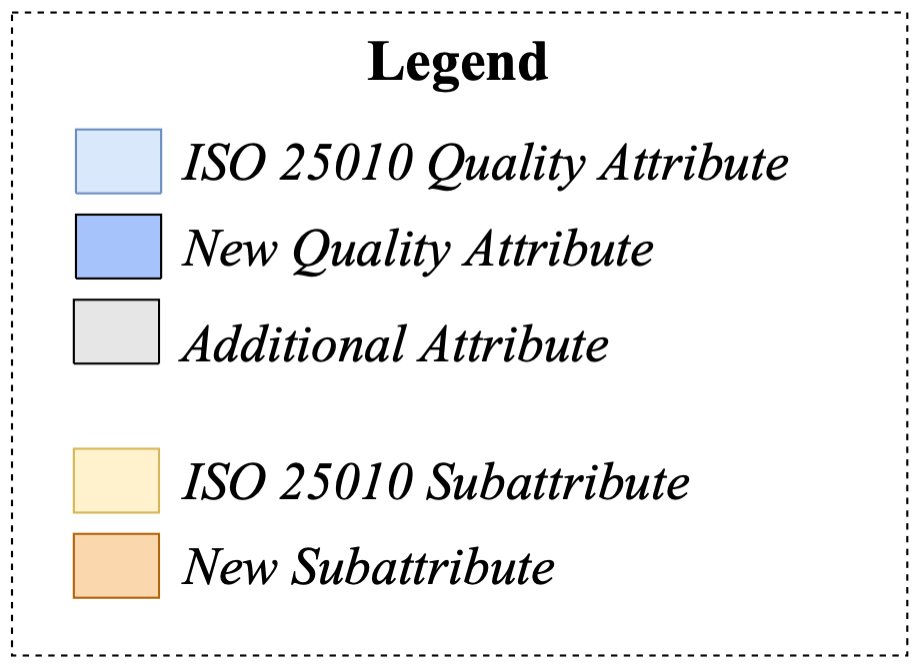
\includegraphics[width=0.4\textwidth]{qas-legend.drawio}
	\caption[Spezielle \acrlongpl{qa} für Microservices-Architekturen]{
		Spezielle \acrfullpl{qa} für Microservices-Architekturen nach \Citet{master-daniel-koch}.
	}
	\label{fig:qas}
\end{figure}
Dabei handelt es sich zu großen Teilen um die nach der Literaturrecherche wichtigsten \glspl{qa} aus der ISO 25010~\cite{ISO-25010}, die durch wenige Microservices-spezifische \glspl{qa} ergänzt wurden.
Abgesehen davon, dass diese besser an die Architektur angepasst sind, ist es notwendig, diese zu verwenden, da der \gls{arh} nur diese zur Auswahl hat.

Die letzte Anpassung betrifft die zusätzliche Priorisierung der Szenarien.
In der Vorlage von \Citet{SVAHNBERG20071893} ist keine explizite Bewertung oder Priorisierung der Szenarien gegeben.
Das ist aufgrund des Kontexts der qualitativen Bewertung durch Menschen auch nicht nötig.
Im Vergleich dazu können bei der automatisierten Auswertung durch ein Werkzeug wie den \gls{arh} die Szenarien nicht automatisch eingeschätzt werden.
Aus diesem Grund erfolgt in Schritt 3 zusätzlich eine dreistufige Bewertung der Szenarien hinsichtlich ihrer Wichtigkeit und technische Schwierigkeit.
Die Bewertung erfolgt von A-C, wobei A für sehr wichtig und sehr technisch schwierig steht.

Eine Übersicht über die beschriebene Methodik ist in \cref{tab:architekturreview-plan} zu finden.

\begin{table}[!h]
  \centering
  \begin{tabular}{m{4cm} m{8cm} p{1.3cm}}
    \toprule
    \textbf{Schritt nach \Citet{SVAHNBERG20071893}} & \textbf{Sub-Schritt} & \textbf{Zeit} \\ \midrule
    1. Einleitung in die Me\-tho\-dik & & 10 min\\ \hline
    \multirow{2}{=}[0cm]{2. Identifikation von Qualitätsanforderungen} & Umfrage über wichtigste drei Sub-\glspl{qa} &  \multirow{3}{=}[0.2cm]{20 min}\\
    & Diskussion über Priorisierung der Sub-\glspl{qa} & \\ \hline
    \multirow{3}{=}[-0.3cm]{3. Szenarienerhebung} & Erstellen Szenarien zu wichtigsten Sub-\glspl{qa}& \multirow{3}{=}[-0.3cm]{60 min}\\
    & Hinzufügen Wichtigkeit \& Technische Schwierigkeit zu Szenarien  & \\
    & Szenarien mit weiteren \glspl{qa} assoziieren  & \\ \hline
    5. Szenario- und Archi\-tek\-turanalyse & Architekturbewertung anhand der Szenarien & 10 min \\
    \bottomrule
  \end{tabular}
  \caption[Zeitplan für das Architekturreview]{
    Zeitplan für das Architekturreview in Phase 1 dieser Thesis.
  }
  \label{tab:architekturreview-plan}
\end{table}


\subsection{Strukturierte Feldnotizen}
\label{sec:structured-field-notes}

Während Phase 1 also in einer Fokusgruppe durchgeführt wurde, findet die Bearbeitung in den folgenden Phasen größtenteils in Einzelarbeit statt.
Um dabei strukturiert zu protokollieren, welche Aktivitäten im Rahmen dieser Phasen durchgeführt wurden, werden systematisch durchgeführte Aktivitäten mit gemachten Erfahrungen und Herausforderungen dokumentiert und am Ende ausgewertet.
Dazu werden strukturierte Feldnotizen verwendet~\cite{seaman2008qualitative}.
Dabei können die involvierten Stakeholder zur Rate gezogen werden.


\section{Evaluation des \gls{mmf}}

Das bis inklusive Phase 3a geplante Refactoring soll dann in Phase 3b im Rahmen eines minimalen Prototyps umgesetzt und simuliert werden, da ein Refactoring des kompletten Systems im zeitlichen Rahmen dieser Arbeit nicht möglich wäre.
Dabei entstehende Prototypen könnten Vorläufer von \emph{jadice flow 2.0} werden.

Im Nachgang sollen die Ergebnisse dieses Experiments ausgewertet werden. Um quantitativ vergleichbare Ergebnisse zu erhalten, sollen im Vorlauf des Experiments Vergleichskriterien und Messmethoden definiert werden, die es möglich machen, gleichartige Anwendungsfälle von \emph{jadice flow 1.0} und neuen Prototypen zu vergleichen.
